\documentclass[12pt,letterpaper]{article}

\usepackage[utf8]{inputenc}
\usepackage{ragged2e}
\usepackage{amsfonts}
\usepackage{amssymb}
\usepackage{graphicx}
\usepackage{multicol}
\usepackage{changepage}
\usepackage{float}
\usepackage{cite}
\usepackage{url}
\usepackage[left=2.50cm, right=2.50cm]{geometry}
\usepackage[spanish]{babel}
\graphicspath{ {images/} }


\author{Hern\'andez Ceciliano Luis \'Angel}
\title{Entrega 6}
\date {2020-11-24}

\begin{document}
	%encabezado 
	\pagestyle{plain}
	{

		% Imágenes de la portada
		{
			\begin{tabular}
				{
					p{0.75\textwidth} 
					p{0.25\textwidth} 
				}
				
\includegraphics[width=1.5cm, height=2.5cm]{ipn.png} &  
				
\includegraphics[width=2.5cm, height=2cm]{escom.png}
			\end{tabular}
		}

		% Datos de la caratula
		\begin{center}

			\par\vspace{1cm} %Espacio dejado antes del encabezado
			{
				\Huge\textbf
				{
					Instituto Polit\'ecnico Nacional 
					\\[.2cm]Escuela Superior de C\'omputo
				}
			}

			\par\vspace{0.5cm}
			{
				\large\textbf
				{
					Ingenier\'ia en sistemas computacionales 
					\\[.5cm]An\'alisis y diseño orientado a objetos
				}
			}

			\vfill

			\par\vspace{0.7cm}
			{
				\textbf
				{
					Entrega 6 \\
                    CEDAE (Centro dermatológico de alta especialidad)
				}
			}

			\vfill

			\par\vspace{0.7cm}
			{
				\textbf
				{
                    Equipo 3:
                    \\Angeles Hernández Jesús Eduardo
                    \\Chanes Nuñez Ricardo Jehonadab
                    \\García Gamiño Rafael Julian
                    \\Hernández Ceciliano Luis Ángel
                    \\Mendoza Cuellar José Oscar
                    \\Olvera Olvera Kevin Jesús
                    \\Paniagua Juárez Nadia Patricia
                    \\Ramírez Fuentes Edgar Alejandro
                    \\Zamorano Cruz Juan Raymundo
					\\2CV9
				} 
			}

			\par\vspace{3cm}

		\end{center}
		\clearpage
	}

	\newpage
	\tableofcontents
    \newpage

    \newpage
    
    \section{Objetivo}
    El proposito de este documento es mostrar al lector la organización, especificaciones y diseños para el sistema web de CEDAE.

    \section{Organización del SCRUM Team}
    \justify
                Después de una reunión enfocada a la selección de los roles que tendrá cada integrante del equipo, se llegó a la siguiente
                organización.
                \\\\
                \begin{itemize}
                    \item Product Owner - M.C. Maldonado Castillo Idalia 
                    \item SCRUM Master - Hernández Ceciliano Luis Ángel 
                    \item Development team
                        \begin{itemize}
                            \item Equipo de análisis
                                \begin{itemize}
                                    \item Angeles Hernández Jesús Eduardo
                                    \item Hernández Ceciliano Luis Ángel
                                \end{itemize}
                            \item Equipo de diseño
                            \begin{itemize}
                                \item Panigua Juárez Nadia Patricia
                                \item Zamorano Cruz Juan Raymundo
                            \end{itemize}
                            \item Equipo de desarrollo
                            \begin{itemize}
                                \item Bases de Datos
                                    \begin{itemize}
                                        \item Mendoza Cuellar José Oscar
                                        \item Olvera Olvera Kevin Jesús
                                    \end{itemize}
                                \item Front-end
                                \begin{itemize}
                                    \item Ramírez Fuentes Edgar Alejandro
                                    \item Panigua Juárez Nadia Patricia
                                    \item Zamorano Cruz Juan Raymundo
                                \end{itemize}
                                \item Back-end
                                \begin{itemize}
                                    \item Chanes Nuñez Ricardo Jehonadab
                                    \item García Garmiño Rafael Julian
                                    \item Ramírez Fuentes Edgar Alejandro
                                \end{itemize}
                            \end{itemize}
                        \end{itemize}
                \end{itemize}

    \section{Acuerdos del SCRUM Team}
    \justify
                En una de las reuniones diarias del SCRUM se llegaron a
                los siguientes acuerdos, los cuales deberán ser cumplidos de 
                manera exacta.
                \begin{itemize}
                    \item Daily standup meetings
                    \begin{itemize}
                        \item Las daily meeting se realizarán de Lunes a Viernes en un horario de 22:00 a 22:18 
                        \item Cada participante tendrá 2 minutos para hablar
                        \item Cada integrante deberá tener listos los puntos a tratar antes de la reunión para evitar prolongar la reunión
                        \item No se tendrá tolerancia ante retardos
                        \item Si un integrante tiene más de cinco faltas en estas reuniones, se expulsará del equipo por falta de compromiso con el proyecto
                        \item Solo se tocarán temas con respecto a actividades realizadas el día de la reunión y obstáculos que se tienen para la realización de futuras actividades
                        \item Si los equipos desean reunirse por su parte para tratar dudas acerca del proyecto, son libres de hacerlo.
                    \end{itemize}
                    \item Sprint planning meetings, Sprint review meeting y Sprint retrospective meeting
                    \begin{itemize}
                        \item Este tipo de reuniones se realizarán en los días sabádos a las 22:00 para la dedicación de tiempo necesario.
                        \item No habrá tolerancia ante retrasos en este tipo de reuniones
                        \item No habrá tolerancia ante ausencia en este tipo de reunión. Si algún integrante llega a faltar, se pondrá a votación su estancia en el equipo de trabajo 
                        \item La duración de la reunión será dependiente del entendimiento organización, opiniones del equipo acerca del proyecto 
                    \end{itemize}
                \end{itemize}

    \section{Descripción del proyecto}
    \justify
                Se desarrollará un sistema web el cual apoyará a la clínica CEDAE a la gestión de doctores titulares,
                doctores auxiliares, trabajadores de la clínica, pacientes, stock de medicina, citas médicas, expedientes médicos,
                recetas médicas, entre otras futuras funcionalidades.
                Además, se implementarán todos aquellos servicios y subservicios que la clínica CEDAE presta para así lograr satisfacer
                las necesidades del cliente.
                \\\\
                El sistema le permitirá al médico titular visualizar expedientes de sus pacientes, emitir recetas tanto físicas,
                por correo electrónico o por la plataforma web, permitir el acceso a su receta médica de sus pacientes, entre otras futuras funcionalidades.
                \\\\
                El sistema permitirá a los usuarios, únicamente aquellos registrados en la plataforma, visualizar recetas previamente autorizadas por 
                su médico, visualizar futuras citas, entre otras futuras funcionalidades.
                \\\\
                Para el módulo del área de farmacia se llevará el control de los medicamentos en stock, se dará alerta de aquellos medicamentos que estén cerca de incumplimiento 
                de normas de COFEPRIS para así ayudar al cliente a priorizar la venta de medicamento cercano a ser desechado, entre otras futuras funcionalidades.
                \\\\
                Por parte del sector administrativo de la clínica permitirá generar citas, generar reportes estadísticos que el cliente requiera, entre futuras funcionalidades.
                \\\\
                Nota: La descripción actual del proyecto es con base en la información que hasta el momento se tiene acerca del proyecto.

    \section{Requerimientos del proyecto}
        \justify
                \begin{itemize}
                    \item Requerimientos funcionales
                    \begin{enumerate}
                        \item El sistema permitirá a cada usuario iniciar y cerrar sesión en el sistema.
                        \item El sistema permitirá al usuario administrador registrar otros usuarios.
                        \item El sistema permitirá al usuario administrador dar de baja a otros usuarios.
                        \item El sistema permitirá al usuario administrador modificar la información de otros usuarios.
                        \item El sistema permitirá al usuario recepcionista agendar citas para pacientes.
                        \item El sistema permitirá al paciente consultar las fechas de sus citas a través de su cuenta.
                        \item El sistema permitirá al médico titular generar recetas médicas.
                        \item El sistema permitirá al médico titular generar o hacer cambios al expediente clínico de pacientes.
                        \item El sistema permitirá a los médicos titulares y auxiliares consultar expedientes clínicos de sus pacientes.
                        \item El sistema permitirá al paciente consultar su expediente clínico a través de su cuenta.
                        \item El sistema permitirá al médico titular habilitar los expedientes clínicos para su consulta por parte del usuario.
                        \item El sistema permitirá al usuario administrador generar de reportes estadísticos.
                        \item El sistema contará con manejo de almacén de farmacia.
                        \item El sistema permitirá a los médicos consultar la disponibilidad de medicamentos en farmacia.
                        \item El sistema permitirá al encargado de farmacia consultar la disponibilidad de medicamentos.
                        \item El sistema generará una advertencia para los usuarios encargados de farmacia cuando un medicamento esté pronto a caducar o infringir las normas de COFEPRIS.
                        \item El sistema permitirá a los médicos generar recetas físicas y electrónicas (Vistas en sistema o enviadas por correo electrónico).
                        \item El sistema permitirá llevar un registro del personal que atendió al paciente para cada consulta que este tuvo.
                        \item El sistema permitirá agendar citas a usuarios sin registro.
                        \item Las citas solo podrán ser agendadas en el calendario en tiempos de 30 minutos durante el horario de atención.
                        \item La duración de las citas de primera vez será de 1 hora.
                        \item La duración de las citas  subsecuentes será de 30 minutos.
                        \item Cuando se agenda una cita de primera vez en línea, el usuario no podrá escoger el médico que lo atenderá, solo el horario.
                        \item Cuando se agenda una cita de primera vez ya sea de manera presencial o telefónica, el usuario podrá elegir el médico y el horario de su cita.
                        \item El sistema enviará correos electrónicos para confirmación de las citas.
                        \item El sistema permitirá al usuario recepcionista consultar la agenda de cada médico titular.
                        \item El sistema permitirá al usuario recepcionista ver las citas de todos los usuarios.
                        \item El sistema permitirá al usuario recepcionista realizar cobros de consultas.
                        \item El sistema permitirá al encargado de farmacia realizar cobros por medicamentos.
                        \item El sistema permitirá al encargado de farmacia modificar la existencia de medicamentos en inventario.
                    \end{enumerate}
                    \item Requerimientos no funcionales
                    \begin{enumerate}
                        \item Los expedientes clínicos serán generados con base en la norma NOM-024-SSA3-2010.
                        \item El surtido de recetas por parte de la farmacia se debe apegar al Artículo 226 de la Ley General de Salud.
                        \item El sistema no permitirá agendar cita con un médico en específico en su horario de comida.
                        \item El sistema será completamente funcional en el navegador Google Chrome en la versión Versión 86.0.4240.183 (Build oficial) o posterior.
                        \item El sistema debe tener una disponibilidad del 99 porciento de las veces en que un usuario intente accederlo.
                        \item El sistema debe proporcionar mensajes de error que sean informativos y orientados a usuario final.
                        \item El sistema debe poseer interfaces gráficas bien formadas.
                        \item El promedio de duración de fallas no podrá ser mayor a 15 minutos.
                        \item El tiempo para iniciar o reiniciar el sistema no podrá ser mayor a cinco minutos.
                        \item El sistema debe manejar fuentes del alfabeto Español.
                    \end{enumerate}
            \end{itemize}
            Nota: Los siguientes requirimientos están sujetos a cambios, por lo cual no se deberán tomar como requerimientos finales.
        \subsection{Reglas del negocio}
            \begin{enumerate}
                \item El paciente podrá ver su expediente médico únicamente si ha pedido autorización.
                \item Las caducidades de medicamentos serán tratadas conforme a las normas de la COFEPRIS.
                \item Se debe de cumplir con la Ley Federal de Protección de Datos Personales en Posesión de los Particulares para los datos almacenados de los usuarios.
                \item La clínica atenderá en un horario de Lunes a Viernes de 10:00 a 20:00 horas.
                \item Los médicos tienen un horario fijo, en el cual se contemplan sus horas de comida.
            \end{enumerate}

    \section{Casos de uso}
        \justify
            \subsection{Casos de uso por modulo del sistema}
                \subsubsection{Modulo de gestión de usuarios}
                    \begin{itemize}
                        \item CUGU1.1 Iniciar sesión 
                        \item CUGU1.2 Ver perfil
                        \item CUGU1.3 Cerrar sesión 
                        \item CUGU1.4 Cambiar contraseña 
                        \item CUGU1.5 Registrar usuario 
                        \item CUGU1.6 Eliminar usuario 
                        \item CUGU1.7 Modificar información 
                        \item CUGU1.8 Ver usuarios registrados 
                        \item CUGU1.9 Ver paciente 
                    \end{itemize}
                \subsubsection{Modulo de inventario}
                    \begin{itemize}
                        \item CUIBP1.1 Buscar medicamento 
                        \item CUIBP1.2 Agregar medicamento 
                        \item CUIBP1.3 Eliminar medicamento 
                        \item CUIBP1.4 Ver inventario 
                        \item CUIBP1.5 Notificar stock 
                    \end{itemize}
                \subsubsection{Modulo de expediente}
                    \begin{itemize}
                        \item CUEX1.1 Crear expediente 
                        \item CUEX1.2 Buscar expediente 
                        \item CUEX1.3 Añadir consulta 
                        \item CUEX1.4 Modificar expediente 
                        \item CUEX1.5 Ver expediente 
                        \item CUEX1.6 Eliminar expediente 
                        \item CUEX1.7 Agregar receta
                    \end{itemize}

    \section{Diagramas y especificación de casos de uso}
        \subsection{Diagramas del modulo de gestión de usuarios}
            \begin{figure}[H]
                \centering
                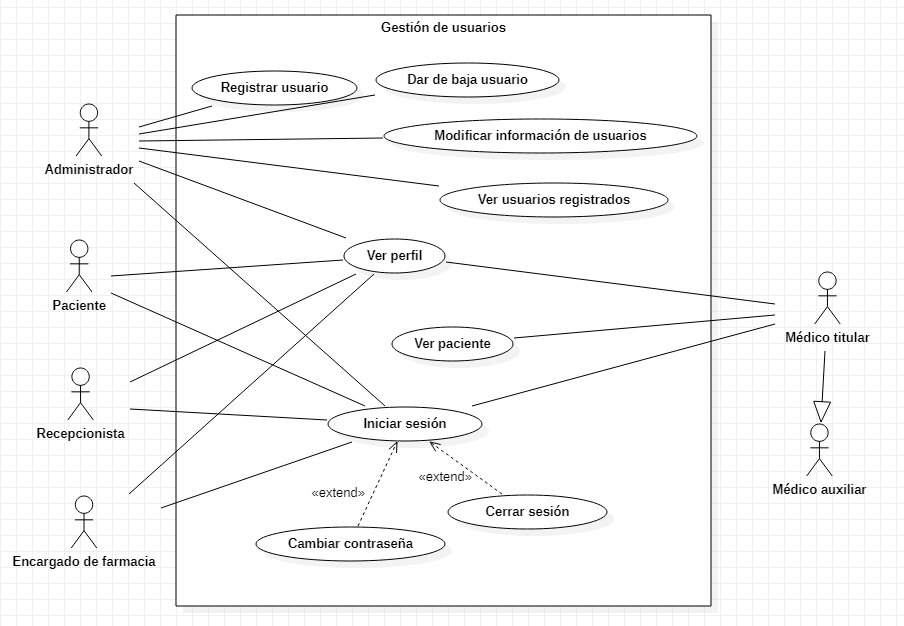
\includegraphics [scale=0.5]{casosUso/gestionUsuarios}
                \caption{Diagrama de gestión de usuarios}
            \end{figure}

            \newpage
            CUGU1.1 Iniciar sesión 
            \begin{figure}[H]
                \centering
                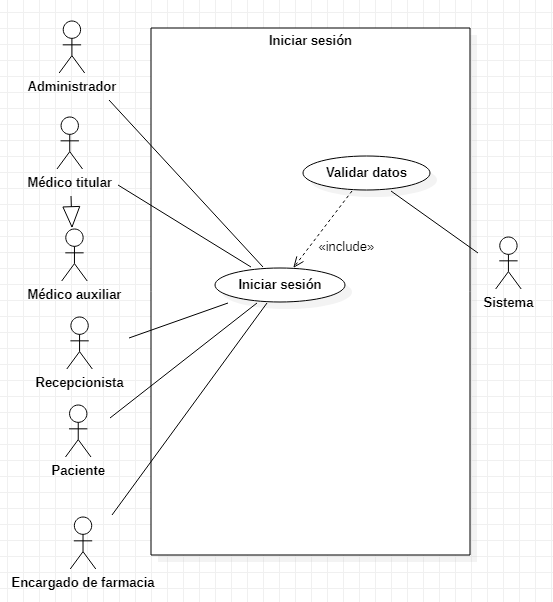
\includegraphics [scale=0.3]{casosUso/iniciarSesion}
                \caption{Diagrama de inicio de sesión}
            \end{figure}
            \begin{figure}[H]
                \centering
                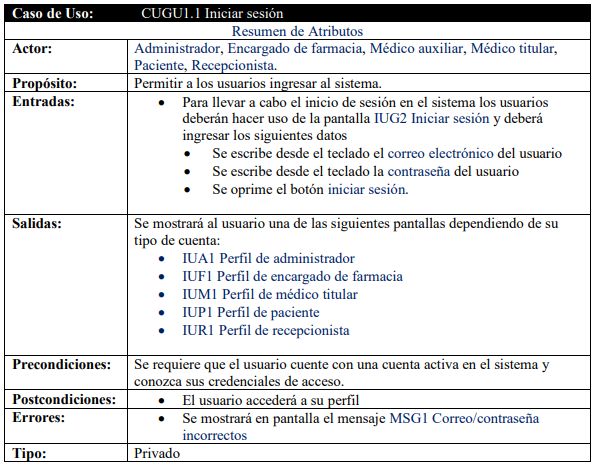
\includegraphics [scale=0.9]{specs/specIniciarSesion}
            \end{figure}
            \begin{figure}[H]
                \centering
                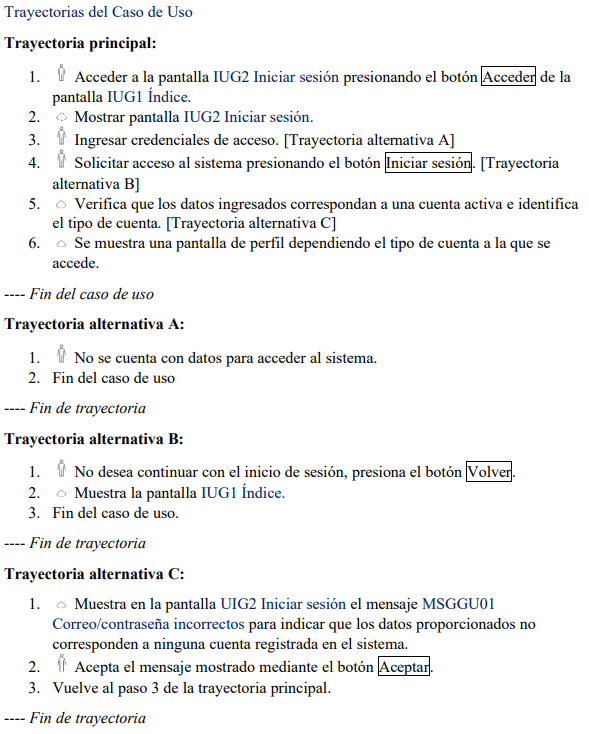
\includegraphics [scale=0.9]{specs/trayIniciarSesion}
            \end{figure}

            \newpage
            CUGU1.2 Ver perfil
            \begin{figure}[H]
                \centering
                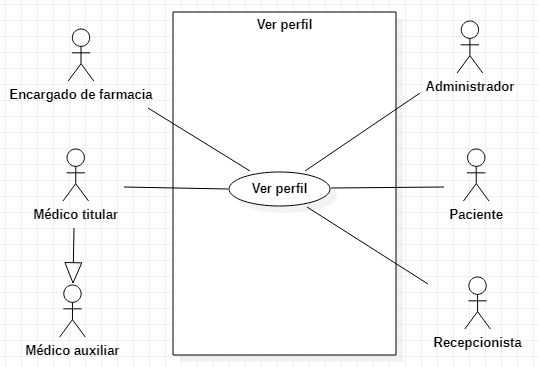
\includegraphics [scale=0.4]{casosUso/verPerfil}
                \caption{Diagrama de visualización de perfil}
            \end{figure}
            \begin{figure}[H]
                \centering
                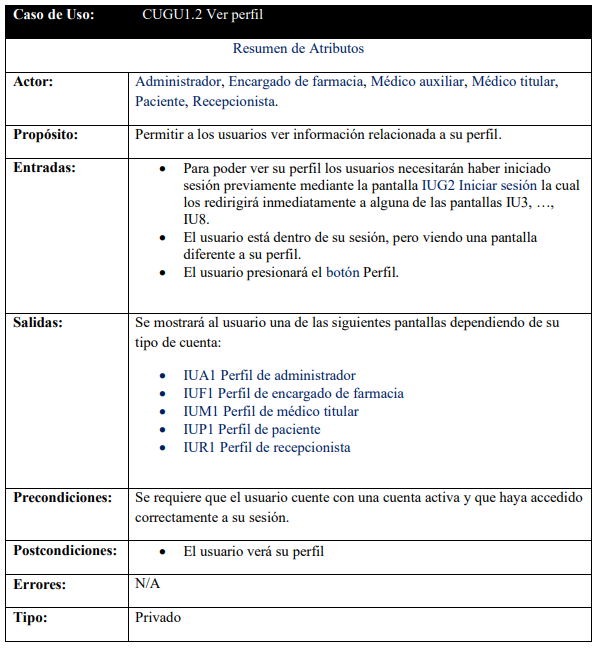
\includegraphics [scale=0.7]{specs/specVerPerfil}
            \end{figure}
            \begin{figure}[H]
                \centering
                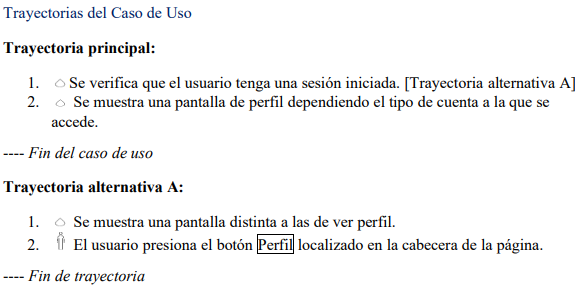
\includegraphics [scale=0.9]{specs/trayVerPerfil}
            \end{figure}

            \newpage
            CUGU1.3 Cerrar sesión 
            \begin{figure}[H]
                \centering
                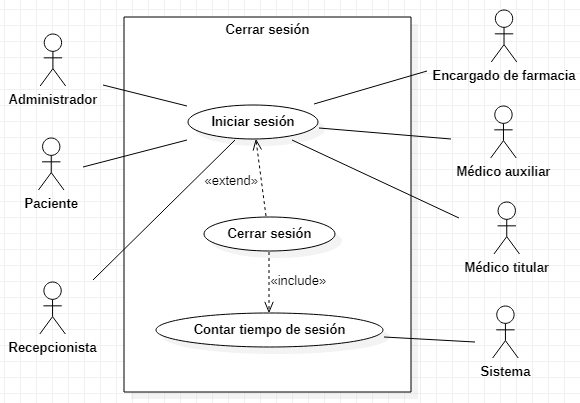
\includegraphics [scale=0.3]{casosUso/cerrarSesion}
                \caption{Diagrama de cerrar sesión}
            \end{figure}
            \begin{figure}[H]
                \centering
                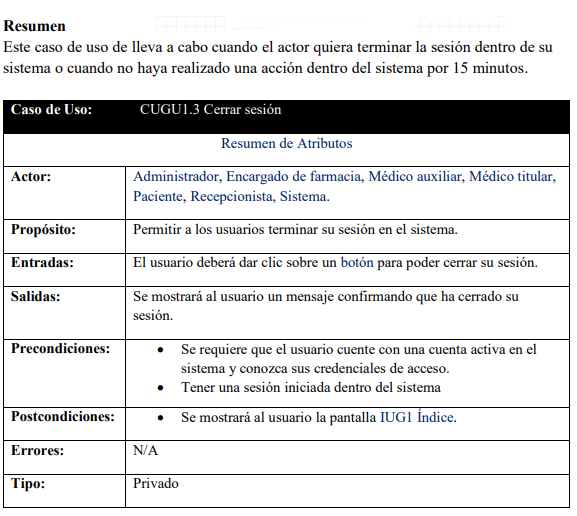
\includegraphics [scale=0.85]{specs/specCerrarSesion}
            \end{figure}
            \begin{figure}[H]
                \centering
                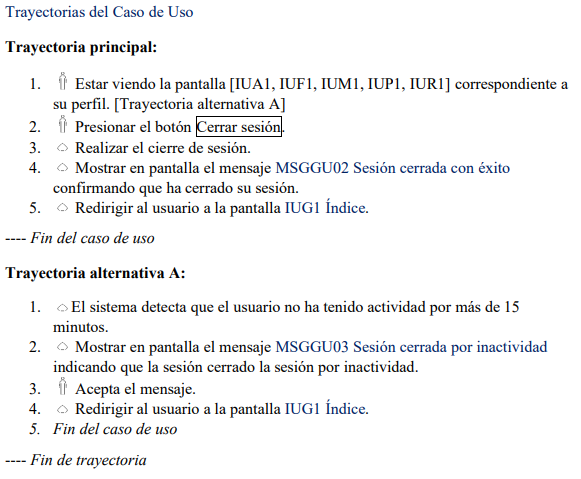
\includegraphics [scale=0.9]{specs/trayCerrarSesion}
            \end{figure}

            \newpage
            CUGU1.4 Recuperar contraseña 
            \begin{figure}[H]
                \centering
                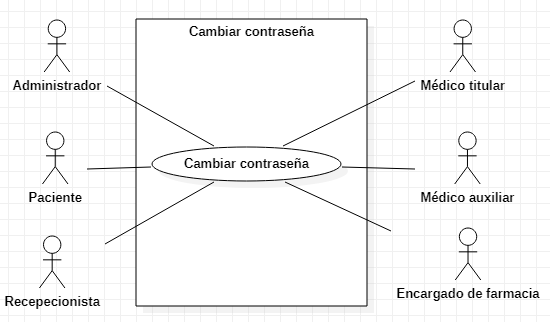
\includegraphics [scale=0.3]{casosUso/recuperarContraseña}
                \caption{Diagrama de cambio de contraseña}
            \end{figure}
            \begin{figure}[H]
                \centering
                \includegraphics [scale=0.75]{specs/specRecuperarContraseña}
            \end{figure}
            \begin{figure}[H]
                \centering
                \includegraphics [scale=0.75]{specs/trayRecuperarContraseña}
            \end{figure}

            \newpage
            CUGU1.5 Registrar usuario 
            \begin{figure}[H]
                \centering
                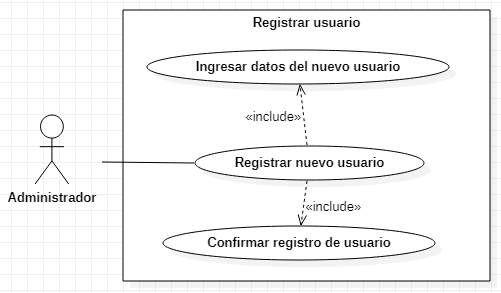
\includegraphics [scale=0.6]{casosUso/registrarUsuario}
                \caption{Diagrama de registro de usuario}
            \end{figure}
            \begin{figure}[H]
                \centering
                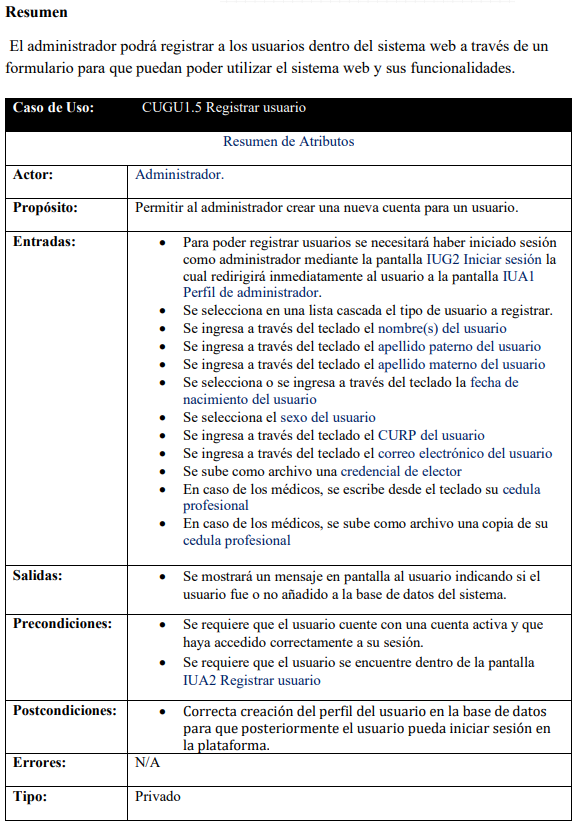
\includegraphics [scale=0.75]{specs/specRegistrarUsuario}
            \end{figure}
            \begin{figure}[H]
                \centering
                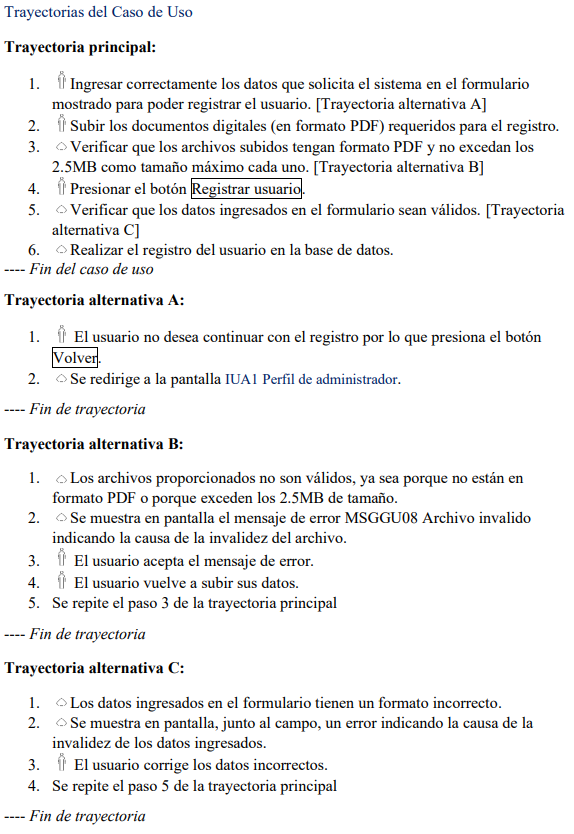
\includegraphics [scale=0.85]{specs/trayRegistrarUsuario}
            \end{figure}

            \newpage
            CUGU1.6 Eliminar usuario 
            \begin{figure}[H]
                \centering
                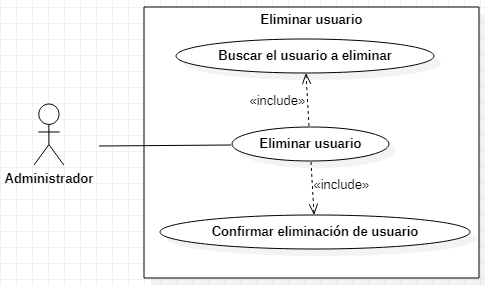
\includegraphics [scale=0.5]{casosUso/eliminarUsuario}
                \caption{Diagrama de eliminar usuario}
            \end{figure}
            \begin{figure}[H]
                \centering
                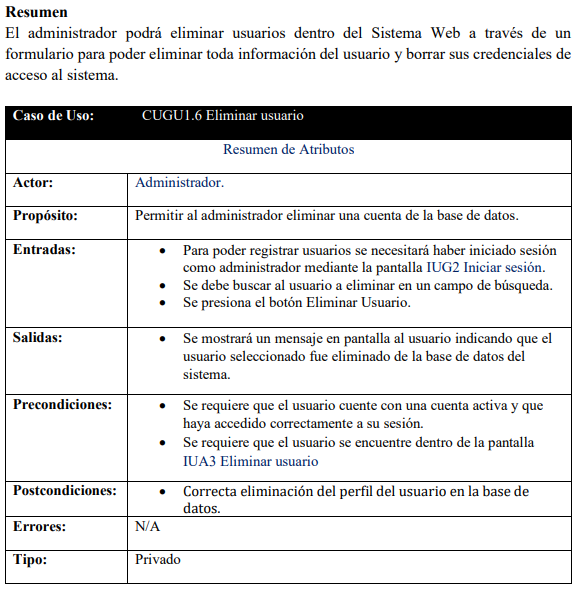
\includegraphics [scale=0.8]{specs/specEliminarUsuario}
            \end{figure}
            \begin{figure}[H]
                \centering
                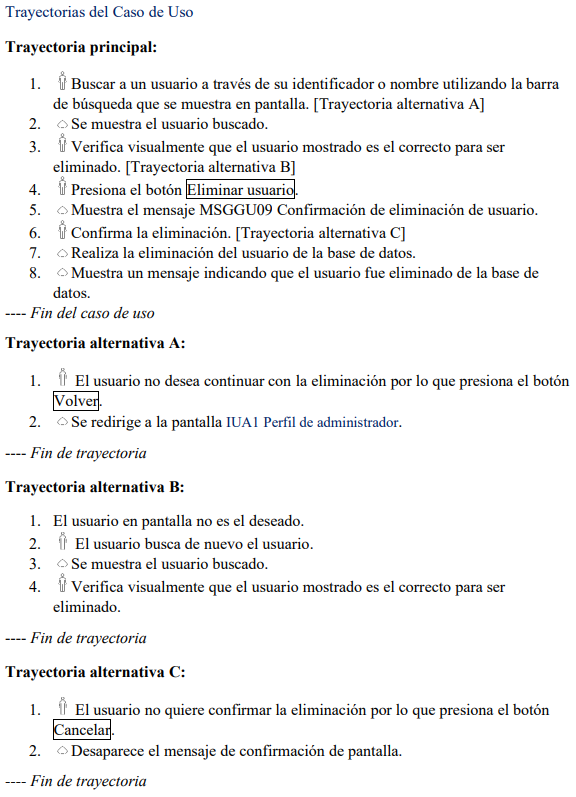
\includegraphics [scale=0.9]{specs/trayEliminarUsuario}
            \end{figure}

            \newpage
            CUGU1.7 Modificar información 
            \begin{figure}[H]
                \centering
                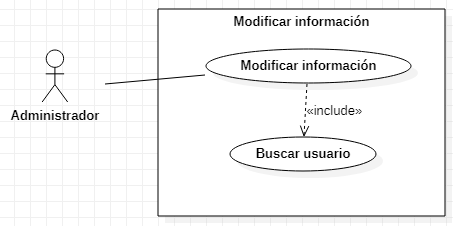
\includegraphics [scale=0.5]{casosUso/modificarInformacion}
                \caption{Diagrama de modificación de información}
            \end{figure}
            \begin{figure}[H]
                \centering
                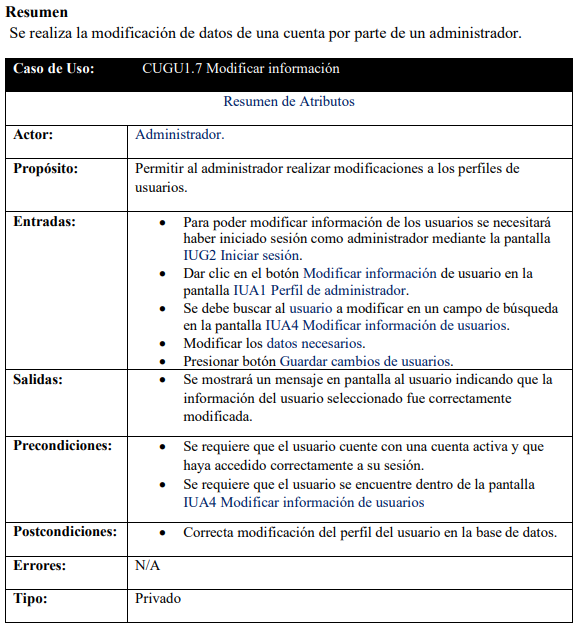
\includegraphics [scale=0.75]{specs/specModificarInformacion}
            \end{figure}
            \begin{figure}[H]
                \centering
                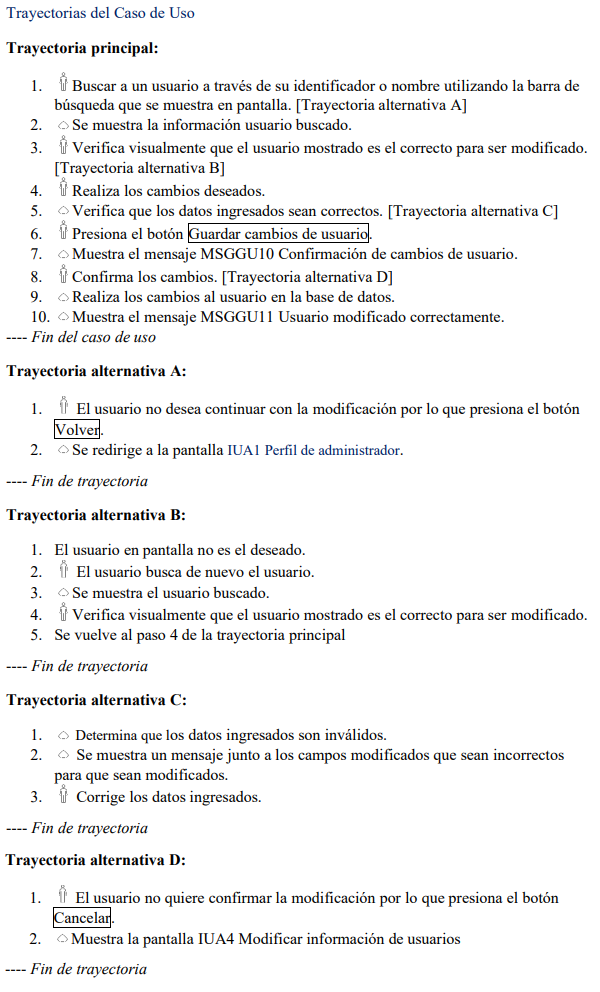
\includegraphics [scale=0.75]{specs/trayModificarInformacion}
            \end{figure}

            \newpage
            CUGU1.8 Ver usuarios registrados 
            \begin{figure}[H]
                \centering
                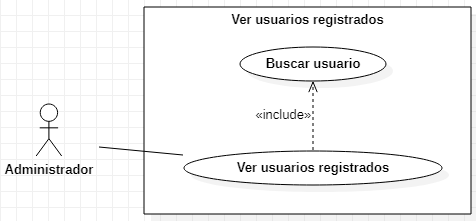
\includegraphics [scale=0.6]{casosUso/verUsuariosRegistrados}
                \caption{Diagrama de visualización de usuarios}
            \end{figure}
            \begin{figure}[H]
                \centering
                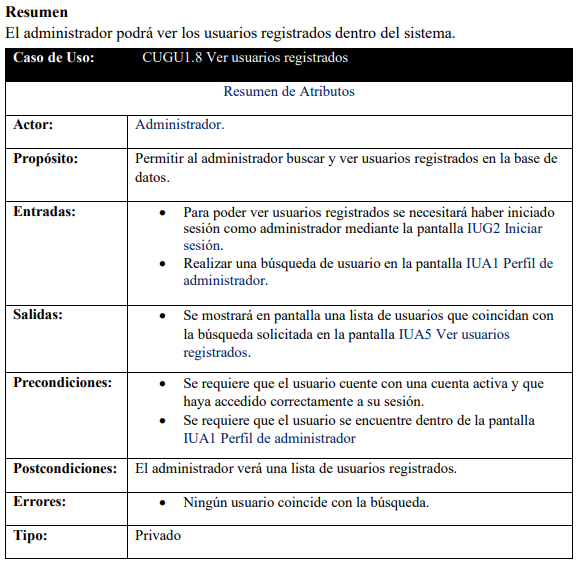
\includegraphics [scale=0.8]{specs/specVerUsuario}
            \end{figure}
            \begin{figure}[H]
                \centering
                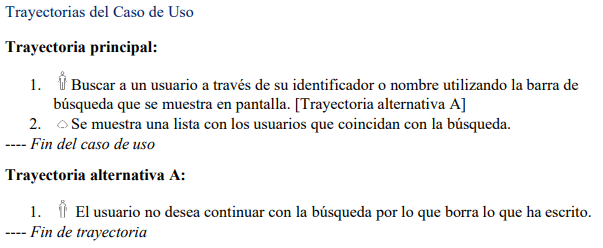
\includegraphics [scale=0.9]{specs/trayVerUsuario}
            \end{figure}

            \newpage
            CUGU1.9 Ver paciente 
            \begin{figure}[H]
                \centering
                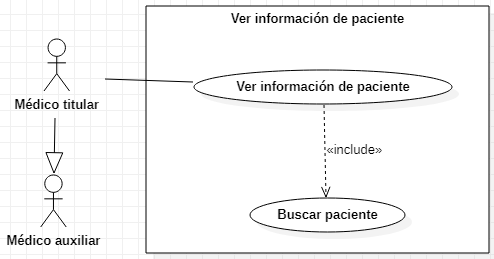
\includegraphics [scale=0.5]{casosUso/verInformacionPaciente}
                \caption{Diagrama de visualización de paciente}
            \end{figure}
            \begin{figure}[H]
                \centering
                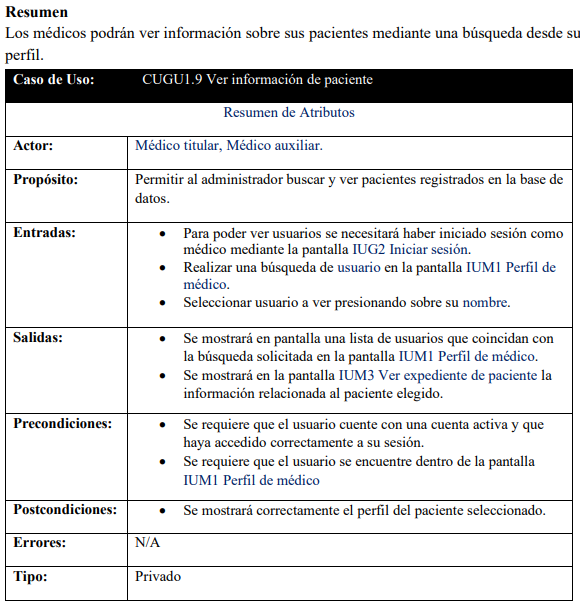
\includegraphics [scale=0.8]{specs/specVerPaciente}
            \end{figure}
            \begin{figure}[H]
                \centering
                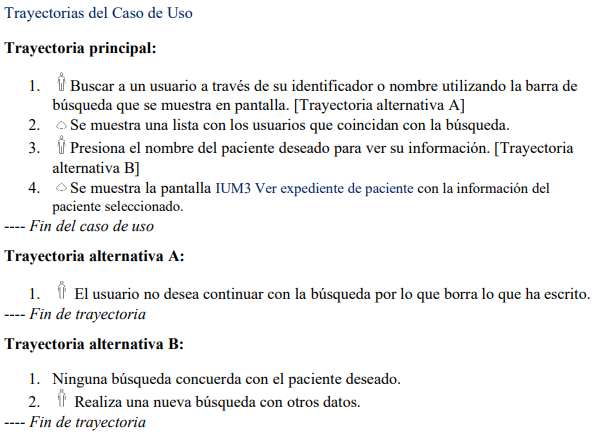
\includegraphics [scale=0.9]{specs/trayVerPaciente}
            \end{figure}
        
            \newpage
        \subsection{Diagramas del modulo de gestión de inventario}
            \begin{figure}[H]
                \centering
                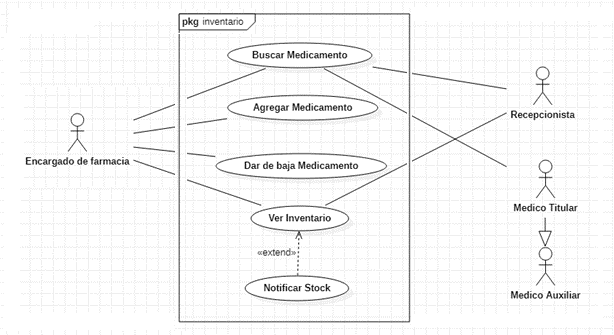
\includegraphics [scale=0.8]{casosUso/gestionInventario}
                \caption{Diagrama de gestión de inventario}
            \end{figure}

            \newpage
            CUIBP1.1 Buscar medicamento 
            \begin{figure}[H]
                \centering
                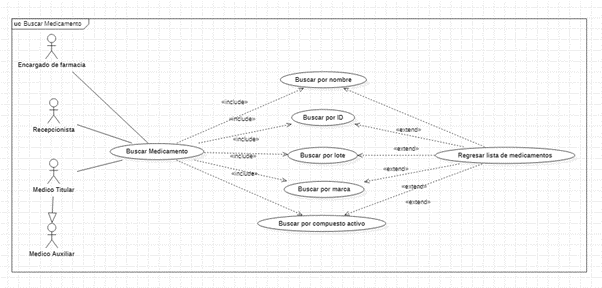
\includegraphics [scale=0.5]{casosUso/buscarMedicamentos}
                \caption{Diagrama de busqueda de medicamento}
            \end{figure}
            \begin{figure}[H]
                \centering
                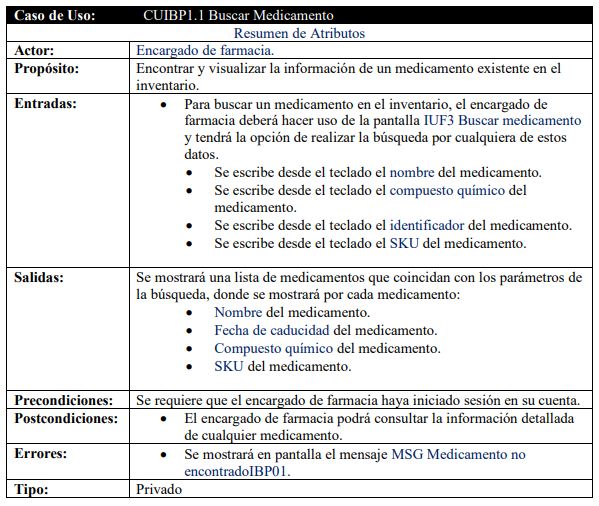
\includegraphics [scale=0.8]{specs/specBuscarMedicamento}
            \end{figure}
            \begin{figure}[H]
                \centering
                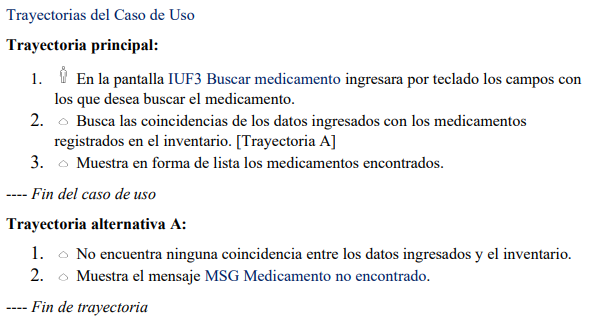
\includegraphics [scale=0.9]{specs/trayBuscarMedicamento}
            \end{figure}

            \newpage
            CUIBP1.2 Agregar medicamento 
            \begin{figure}[H]
                \centering
                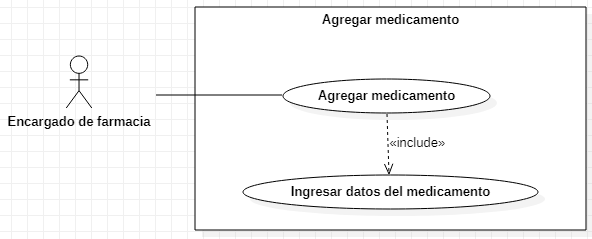
\includegraphics [scale=0.5]{casosUso/agregarMedicamento}
                \caption{Diagrama de agregar medicamento}
            \end{figure}
            \begin{figure}[H]
                \centering
                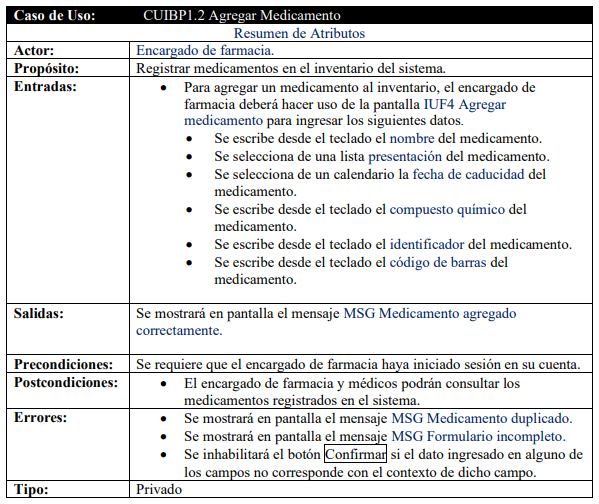
\includegraphics [scale=0.75]{specs/specAgregarMedicamento}
            \end{figure}
            \begin{figure}[H]
                \centering
                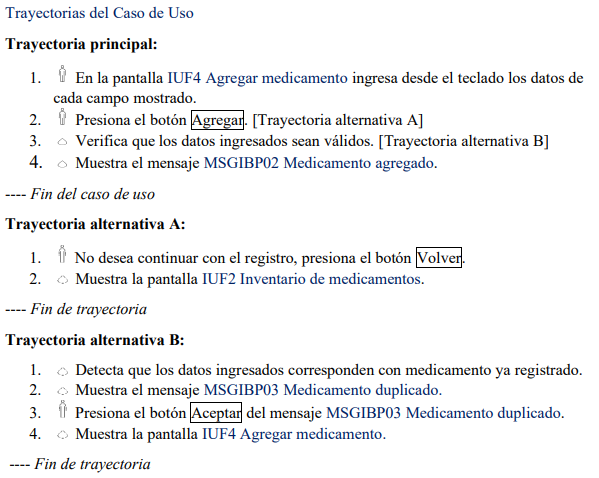
\includegraphics [scale=0.9]{specs/trayAgregarMedicamento}
            \end{figure}

            \newpage
            CUIBP1.3 Eliminar medicamento 
            \begin{figure}[H]
                \centering
                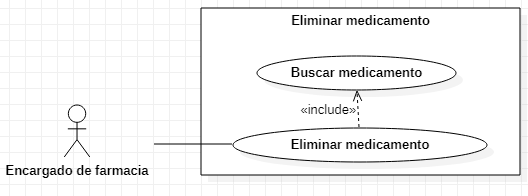
\includegraphics [scale=0.45]{casosUso/eliminarMedicamento}
                \caption{Diagrama de eliminar medicamento}
            \end{figure}
            \begin{figure}[H]
                \centering
                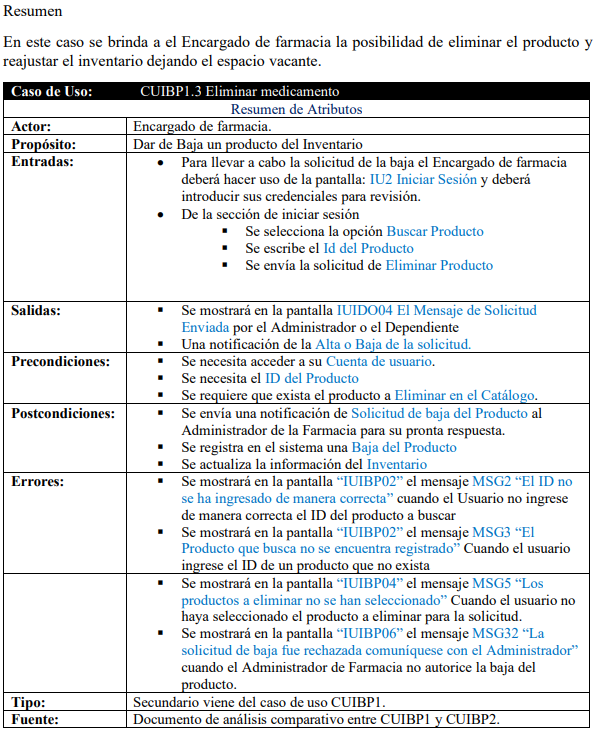
\includegraphics [scale=0.7]{specs/specEliminarMedicamento}
            \end{figure}
            \begin{figure}[H]
                \centering
                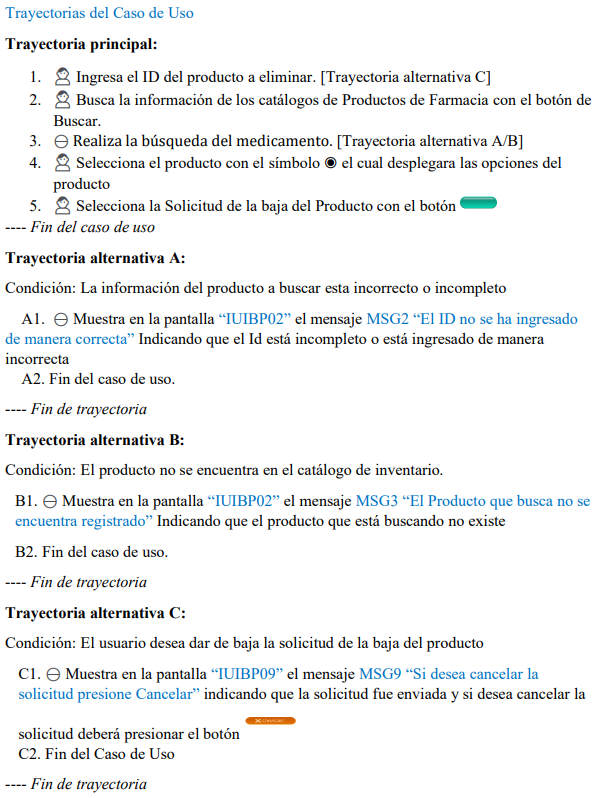
\includegraphics [scale=0.9]{specs/trayEliminarMedicamento}
            \end{figure}

            \newpage
            CUIBP1.4 Ver inventario 
            \begin{figure}[H]
                \centering
                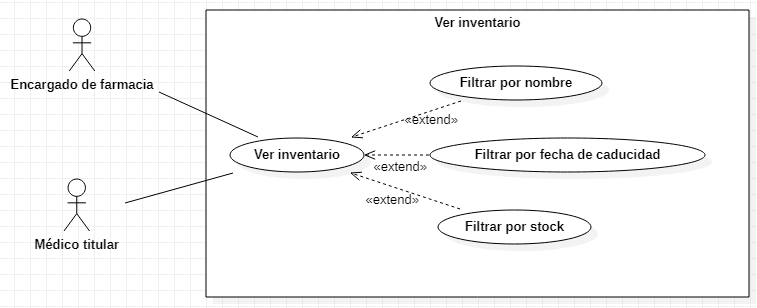
\includegraphics [scale=0.5]{casosUso/verInventario}
                \caption{Diagrama de visualización de inventario}
            \end{figure}
            \begin{figure}[H]
                \centering
                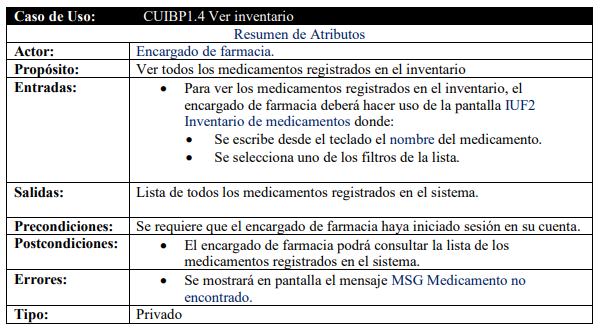
\includegraphics [scale=0.8]{specs/specVerInventario}
            \end{figure}
            \begin{figure}[H]
                \centering
                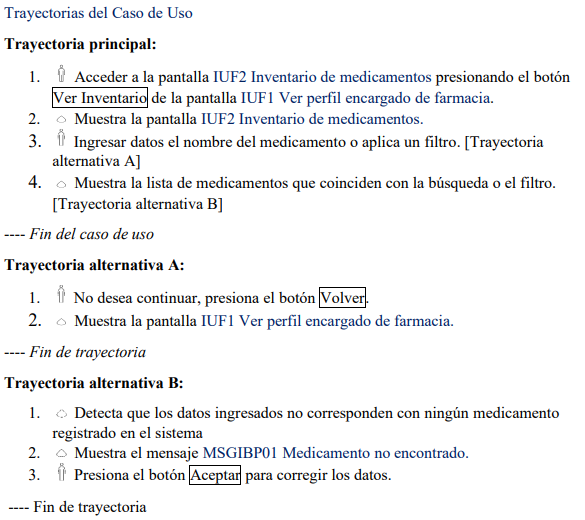
\includegraphics [scale=0.9]{specs/trayVerInventario}
            \end{figure}

             \newpage
            CUIBP1.5 Notificar stock
            \begin{figure}[H]
                \centering
                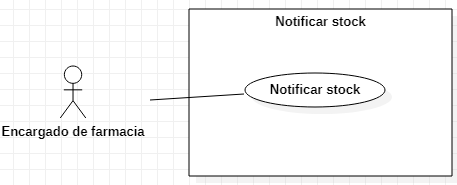
\includegraphics [scale=0.5]{casosUso/notificarStock}
                \caption{Diagrama de notificación de stock}
            \end{figure}
            \begin{figure}[H]
                \centering
                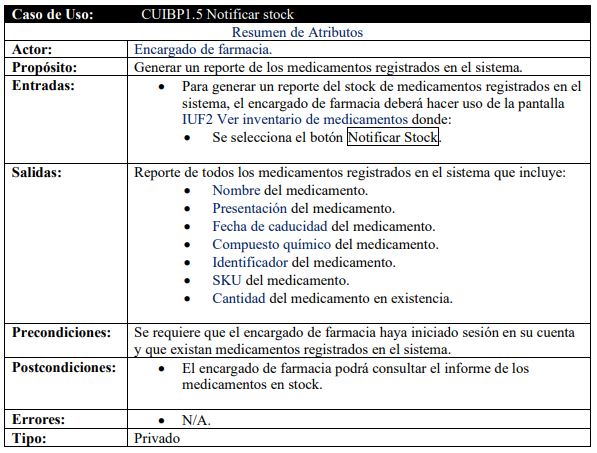
\includegraphics [scale=0.8]{specs/specNotificarStock}
            \end{figure}
            \begin{figure}[H]
                \centering
                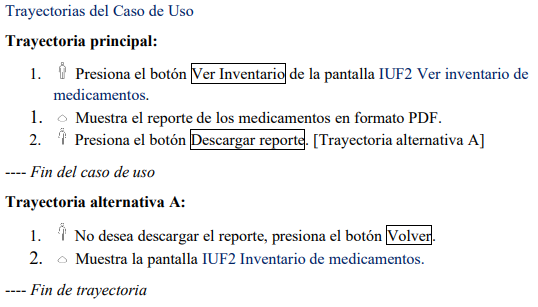
\includegraphics [scale=0.9]{specs/trayNotificarStock}
            \end{figure}

        \newpage
        \subsection{Diagramas del modulo de expediente}
            \begin{figure}[H]
                \centering
                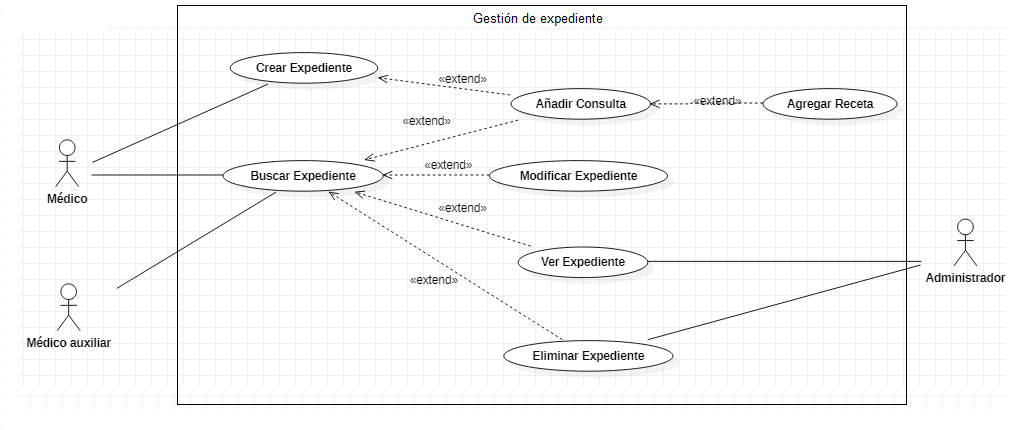
\includegraphics [scale=0.5]{casosUso/gestionExpediente}
                \caption{Diagrama de gestión de expedientes}
            \end{figure}
            \vfill
            
            \newpage
            CUEX1.1 Crear expediente
            \begin{figure}[H]
                \centering
                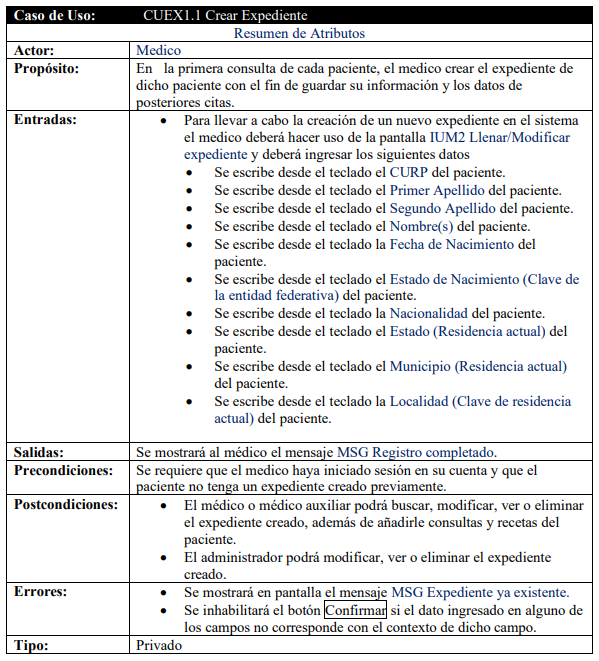
\includegraphics [scale=0.8]{specs/specCrearExpediente}
            \end{figure}
            \begin{figure}[H]
                \centering
                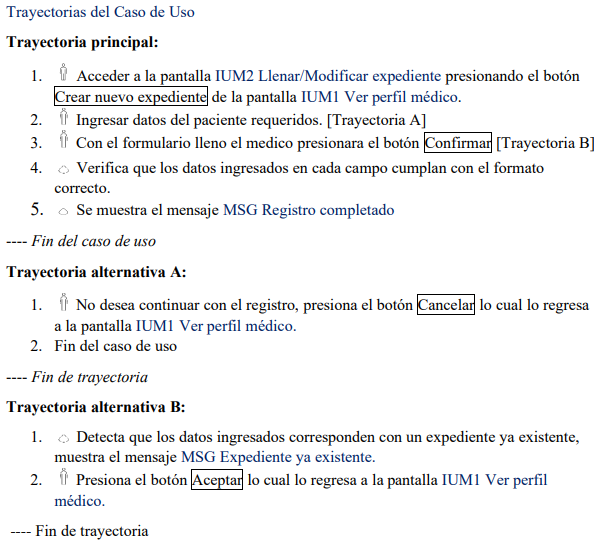
\includegraphics [scale=0.9]{specs/trayCrearExpediente}
            \end{figure}

            \newpage
            CUEX1.2 Buscar expediente 
            \begin{figure}[H]
                \centering
                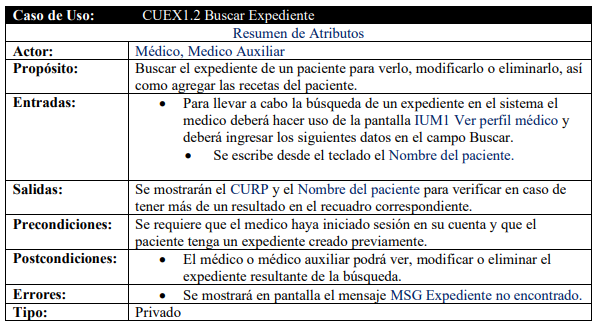
\includegraphics [scale=0.8]{specs/specBuscarExpediente}
            \end{figure}
            \begin{figure}[H]
                \centering
                \includegraphics [scale=0.9]{specs/trayBuscarExpediente}
            \end{figure}

            \newpage
            CUEX1.4 Modificar expediente 
            \begin{figure}[H]
                \centering
                \includegraphics [scale=0.8]{specs/specModificarExpediente}
            \end{figure}
            \begin{figure}[H]
                \centering
                \includegraphics [scale=0.9]{specs/trayModificarExpediente}
            \end{figure}

            \newpage
            CUEX1.5 Ver expediente 
            \begin{figure}[H]
                \centering
                \includegraphics [scale=0.8]{specs/specVerExpediente}
            \end{figure}
            \begin{figure}[H]
                \centering
                \includegraphics [scale=0.9]{specs/trayVerExpediente}
            \end{figure}

            \newpage
            CUEX1.6 Eliminar expediente 
            \begin{figure}[H]
                \centering
                \includegraphics [scale=0.8]{specs/specEliminarExpediente}
            \end{figure}
            \begin{figure}[H]
                \centering
                \includegraphics [scale=0.75]{specs/trayEliminarExpediente}
            \end{figure}

            \newpage
            CUEX1.7 Agregar receta
            \begin{figure}[H]
                \centering
                \includegraphics [scale=0.8]{specs/specAgregarReceta}
            \end{figure}
            \begin{figure}[H]
                \centering
                \includegraphics [scale=0.7]{specs/trayAgregarReceta}
            \end{figure}


    \newpage
    \section{Interfaces del sistema}
        \subsection{Mockups generales}
        IUG1 índice
            \begin{figure}[H]
                \centering
                \includegraphics [scale=0.15]{interfaces/gen_index}
                \caption{Interfaz de página principal}
            \end{figure}
        IUG2 Iniciar sesión
            \begin{figure}[H]
                \centering
                \includegraphics [scale=0.2]{interfaces/gen_login}
                \caption{Interfaz de inicio de sesión}
            \end{figure}
        IUG3 Recuperar contraseña
            \begin{figure}[H]
                \centering
                \includegraphics [scale=0.16]{interfaces/gen_recovery}
                \caption{Interfaz de recuperación de contraseña}
            \end{figure}

        \subsection{Mockups de administrador}
        IUA1 Perfil de administrador
            \begin{figure}[H]
                \centering
                \includegraphics [scale=0.2]{interfaces/adm_perfil}
                \caption{Interfaz de perfil de administrador}
            \end{figure}
        IUA2 Registrar usuario
            \begin{figure}[H]
                \centering
                \includegraphics [scale=0.2]{interfaces/adm_reg_usuario}
                \caption{Interfaz de registro de usuario}
            \end{figure}
        IUA3 Eliminar usuario
            \begin{figure}[H]
                \centering
                \includegraphics [scale=0.2]{interfaces/adm_baja_usuario}
                \caption{Interfaz de baja de usuario}
            \end{figure}
        IUA4 Modificar información de usuarios
            \begin{figure}[H]
                \centering
                \includegraphics [scale=0.2]{interfaces/adm_mod_info}
                \caption{Interfaz de modificación de información de usuario}
            \end{figure}
        IUA5 Ver usuarios registrados
            \begin{figure}[H]
                \centering
                \includegraphics [scale=0.2]{interfaces/adm_ver_usuario}
                \caption{Interfaz de usuarios registrados}
            \end{figure}

        \subsection{Mockups de encargado de farmacia}
        IUF1 Perfil de encargado de farmacia
            \begin{figure}[H]
                \centering
                \includegraphics [scale=0.19]{interfaces/far_perfil}
                \caption{Interfaz de perfil de encargado de farmacia}
            \end{figure}
        IUF2 Inventario de medicamentos
            \begin{figure}[H]
                \centering
                \includegraphics [scale=0.18]{interfaces/far_inv_medicamento}
                \caption{Interfaz de inventario}
            \end{figure}
        IUF3 Buscar medicamentos
            \begin{figure}[H]
                \centering
                \includegraphics [scale=0.20]{interfaces/far_bus_medicamento}
                \caption{Interfaz de busqueda de medicamentos}
            \end{figure}
        IUF4 Agregar medicamentos
            \begin{figure}[H]
                \centering
                \includegraphics [scale=0.2]{interfaces/far_add_medicamento}
                \caption{Interfaz de agregar medicamentos}
            \end{figure}
        IUF5 Eliminar medicamentos
            \begin{figure}[H]
                \centering
                \includegraphics [scale=0.2]{interfaces/far_delete_medicamento}
                \caption{Interfaz de eliminar medicamentos}
            \end{figure}
        
        \subsection{Mockups de médico}
        IUM1 Perfil de médico
            \begin{figure}[H]
                \centering
                \includegraphics [scale=0.18]{interfaces/med_perfil}
                \caption{Interfaz de perfil de medico}
            \end{figure}
        IUM2 Modificar expedientes
            \begin{figure}[H]
                \centering
                \includegraphics [scale=0.2]{interfaces/med_mod_expediente}
                \caption{Interfaz de modificación de expedientes}
            \end{figure}
        IUM3 Ver expedientes
            \begin{figure}[H]
                \centering
                \includegraphics [scale=0.2]{interfaces/med_ver_expediente}
                \caption{Interfaz de visualización de expedientes}
            \end{figure}
        IUM4 Citas agendadas
            \begin{figure}[H]
                \centering
                \includegraphics [scale=0.2]{interfaces/med_ver_citas}
                \caption{Interfaz de citas agendadas}
            \end{figure}
        IUM5 Crear recetas
            \begin{figure}[H]
                \centering
                \includegraphics [scale=0.2]{interfaces/med_crear_receta}
                \caption{Interfaz de creación de recetas}
            \end{figure}

        \subsection{Mockups de paciente}
        IUP1 Perfil de paciente
            \begin{figure}[H]
                \centering
                \includegraphics [scale=0.19]{interfaces/pac_perfil}
                \caption{Interfaz de perfil de paciente}
            \end{figure}
        IUP2 Agendar cita por primera vez
            \begin{figure}[H]
                \centering
                \includegraphics [scale=0.18]{interfaces/pac_cita_primera}
                \caption{Interfaz de agendar primera cita}
            \end{figure}
        IUP3 Agendar cita no por primera vez
            \begin{figure}[H]
                \centering
                \includegraphics [scale=0.18]{interfaces/pac_cita_no_primera}
                \caption{Interfaz de agendar cita}
            \end{figure}
        IUP4 Citas agendadas
            \begin{figure}[H]
                \centering
                \includegraphics [scale=0.2]{interfaces/pac_citas_agendadas}
                \caption{Interfaz de citas agendadas}
            \end{figure}

        \subsection{Mockups de recepcionista}
        IUR1 Perfil de recepcionista
            \begin{figure}[H]
                \centering
                \includegraphics [scale=0.19]{interfaces/rec_perfil}
                \caption{Interfaz de perfil de recepcionista}
            \end{figure}
        IUR2 Realizar cobros
            \begin{figure}[H]
                \centering
                \includegraphics [scale=0.19]{interfaces/rec_cobro}
                \caption{Interfaz de cobros}
            \end{figure}
        IUR3 Agendar cita
            \begin{figure}[H]
                \centering
                \includegraphics [scale=0.18]{interfaces/rec_agendar_cita}
                \caption{Interfaz de agendar cita}
            \end{figure}
        IUR4 Modificar cita
            \begin{figure}[H]
                \centering
                \includegraphics [scale=0.18]{interfaces/rec_modificar_cita}
                \caption{Interfaz de modificar cita}
            \end{figure}
            
        \newpage
        \section{Mensajes de error}
            \begin{itemize}
                \item MSGEX01 Registro completado.
                \item MSGEX02 Expediente ya existente.
                \item MSGEX03 Expediente no encontrado.
                \item MSGEX04 Cambios guardados.
                \item MSGEX05 Confirmar eliminación
                \item MSGEX06 Expediente eliminado.
                \item MSGEX07 Error eliminación de expediente.
                \item MSGEX08 Expediente no eliminado.
                \item MSGEX09 Expediente no encontrado.
                \item MSGEX10 Receta creada
                \item MSGEX11 Indicaciones requeridas
                \item MSGEX12 Receta no creada.
                \item MSGIBP01 Medicamento no encontrado.
                \item MSGIBP02 Medicamento agregado correctamente.
                \item MSGIBP03 Medicamento duplicado.
                \item MSGIBP04 Formulario incompleto.
            \end{itemize}

\end{document}